\documentclass[12pt]{exam}

\usepackage{amssymb}
\usepackage{mathtools}
\usepackage{algorithm}
\usepackage{algpseudocode}
\usepackage{float}  % Figure placement
\usepackage{minted}  % Code highlighting
\usepackage{tikz}  % Flow chart
\usepackage{lipsum}
\usepackage{xspace}
\usepackage{hyperref}
\usepackage{MnSymbol}
\usepackage{pgffor}
\usepackage{mdframed}
\usepackage{array}



\hypersetup{
    colorlinks = true,
    linkcolor = blue,
    urlcolor  = blue,
    citecolor = blue,
    anchorcolor = blue
}

\newcommand{\hwheaderfooter}[3]{
\pagestyle{headandfoot}
\firstpageheadrule
\firstpageheader{#1}{#2}{#3}
\runningheader{#1}{#2}{#3}
\runningheadrule
\firstpagefooter{}{\thepage}{}
\runningfooter{}{\thepage}{}
}

\newcommand{\latex}{\LaTeX\xspace}

\newcommand{\stars}[1]{%
    \foreach \n in {1,...,#1}{%
        $\filledstar$%
    }%
}

\hwheaderfooter{HW 5}{}{CSCI 406}


\begin{document}
\begin{center}
  \fbox{\fbox{\parbox{\textwidth - 0.2 in}{\centering

{Instructions: Please note that handwritten assignments \textbf{will not be graded}. Use the 
provided \latex template to complete your homework. Please do not alter the order or spacing of 
questions (keep each question on its own page). When you submit to Gradescope, you must mark 
which page(s) correspond to each question. \textbf{You may not receive credit for unmarked 
questions}. \\ When including graphical figures, we encourage the use of tools such as \href{https://dreampuf.github.io/GraphvizOnline/}{graphviz} or packages like \href{https://www.overleaf.com/learn/latex/TikZ_package}{tikz} for simple and complex figures. However, these may be handwritten only if they are neat and legible (as defined by the grader). }\\

}}}
\end{center}

\textbf{List any collaborators (besides TAs or professors) here:}

\begin{questions}

\question[15] [W5] Flow. The registrar at the School of Mimes has an unusual method of registration. Each mime (student) must select 10 pose classes that do not conflict with each other that they'd like to take. Of these, the registrar would like to assign 6 classes to each mime.

There are $n$ mimes and $m$ classes with capacities $C_1, C_2, \dots, C_m$. The registrar wishes to assign all mimes to classes using a flow algorithm.

From the list below, select all of the methods which the registrar could employ, only allowing integer flow amounts on each edge. \textbf{Please write a one sentence explanation for why you either selected or did not select the method.}

Note that these methods do not need to all work together to construct a representative flow network, each just has to be a component of a reasonable one.

$\square$ From the source, add edges with capacity 10 to every mime. \\
$\square$ Draw weight 1 edges from every mime to every pose class they selected. \\
$\square$ To the sink, add edges with capacity $C_k$ from pose class $k$. \\
$\square$ The desired flow amount is $6n$. \\
$\square$ The cut that separates the graph into the sink, and everything else, is necessarily a minimum cut.\\
$\square$ The out-degree of each mime node is 10. \\


\clearpage

\question[20] [W6]
Formula 1 teams are preparing for the upcoming season, and each team needs to sign one driver. Each driver is negotiating contracts with teams and have compiled a list of the specific teams they would like to drive for.

Each driver can sign with only one team, and each team can sign only one driver. Your goal is to maximize the number of valid driver-team pairings given $n$ drivers and $m$ teams.

\begin{parts}

\part[10] Formulate this problem as a maximum bipartite matching problem and describe how you would solve it. Clearly define the bipartite graph representation of the problem and explain how you would determine the maximum matching. 





\part[10]In reality, each Formula 1 team signs two drivers. Each driver can still sign with only one team, but each team can now sign up to two drivers. Your goal is to maximize the number of valid driver-team pairings given $n$ drivers and $m$ teams.

\begin{subparts}    
    \subpart[5] How could you modify the original bipartite graph so that the problem remains a maximum bipartite matching problem?
    
    \subpart[5] Instead of solving this as a bipartite matching problem, how could you reframe it as a network flow problem? Describe the graph construction for a flow network and explain how you would run a maximum flow algorithm to solve the problem.

\end{subparts}


\end{parts}



   \newpage 

   \question[15] [W6] You're currently using a single-core machine, but you want to figure out if it's worth investing in a multi-core machine. You have an application where 40\% of the work the application does can be split across an arbitrary number of processors each doing an equal amount of work. The other 60\% of the work must be done on a single processor. (Equivalently, the application is 40\% parallelizable.) How much speedup will you achieve at each value of $p$ where $p$ is the number of processors? Show your work.



\begin{parts}
\part[5] $p = 2$


\part[5] $p = 4$


\part[5] $p = 100$

\end{parts}
\clearpage

\question[20] The nodes in the DAG (directed acyclic graph) below represent tasks you need to complete. An edge $(u,v)$ means that task $u$ must be completed before task $v$ is started. Each task takes the same amount of time.


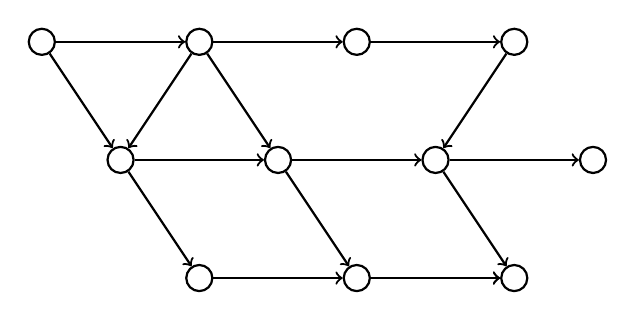
\begin{tikzpicture}[
    ->, % Makes the arrows point to the target node
    % >={Stealth[scale=1.2]}, % Arrow tip style
    thick % Line thickness for arrows
]

% Define the nodes
\node[circle, draw] (A) at (0, 0) {};
\node[circle, draw] (B) at (2, 0) {};
\node[circle, draw] (C) at (4, 0) {};
\node[circle, draw] (D) at (1, -1.5) {};
\node[circle, draw] (E) at (3, -1.5) {};
\node[circle, draw] (F) at (5, -1.5) {};
\node[circle, draw] (K) at (7, -1.5) {};
\node[circle, draw] (G) at (4, -3) {};
\node[circle, draw] (H) at (6, -3) {};
\node[circle, draw] (I) at (2, -3) {};
\node[circle, draw] (L) at (6, 0) {};

% Define the directed edges
\draw (A) edge (B);
\draw (B) edge (C);
\draw (A) edge (D);
\draw (B) edge (D);
\draw (D) edge (E);
\draw (B) edge (E);
\draw (L) edge (F);
\draw (E) edge (F);
\draw (E) edge (G);
\draw (F) edge (H);
\draw (G) edge (H);
\draw (G) edge (H);
\draw (D) edge (I);
\draw (I) edge (G);
\draw (F) edge (K);
\draw (C) edge (L);

\end{tikzpicture}

\begin{parts}
\part[4] What speed up do you get from having 2 people to complete tasks (as opposed to 1)? Two people cannot work together on a single task.


\part[4] What speed up do you get from having 3 people to complete tasks (as opposed to 1)? Two people cannot work together on a single task.

\part[4] What speed up do you get from having infinite people to complete tasks (as opposed to 1)? Two people cannot work together on a single task.


\part[8] How many nodes are in the longest path through the DAG? What does this imply about the maximum speed up?


\end{parts}
\clearpage

\question[25] [W6] The prefix sum, $P$, of a sequence of numbers $X = [x_0, x_1, \dots, x_n]$ is defined as
\[
    P(X) = [(x_0), (x_0 + x_1), (x_0 + x_1 + x_2), \dots, (x_0 + \cdots + x_n)].
\]

\begin{parts}
    \part[5] Provide an efficient non-parallel algorithm for computing the prefix sum of a sequence $X$. (Expected answers are two sentences or less.)

    \part[2] What is the asymptotic complexity of your non-parallel algorithm?


    \part[3] The following pseudocode is for an alternative prefix-sum algorithm:
    
        \begin{algorithm}
        \caption{Alternative Prefix-Sum Algorithm}
        \begin{algorithmic}
            \For{$i \gets 0\ \text{to}\ \left\lfloor \log_2(n) \right\rfloor$}
                \For{$j \gets 0\ \text{to}\ n - 1$}
                    \If{$j < 2^i$}
                        \State $x_j^{i+1} \gets x_j^i$
                    \Else
                        \State $x_j^{i+1} \gets x_j^i + x_{j-2^i}^i$
                    \EndIf
                \EndFor
            \EndFor
        \end{algorithmic}
        \end{algorithm}
        
        The details of the \texttt{if} statement and indexing into $x$ are not important, you can assume that the operations are constant time. What is the time complexity of the alternative algorithm when run on a single processor?


    \part[5] Now, consider Algorithm 1 running on a system with at least $n$ processors. What is the time complexity if we use one processor to perform each of the iterations of the inner \texttt{for} loop?
    


    \part[5] Compute the speedup that Algorithm 1 provides relative to your non-parallel algorithm in parts (a) and (b).


    
    \part[5] Compute the efficiency that Algorithm 1 provides relative to your non-parallel algorithm in parts (a) and (b).


\end{parts}


\clearpage

\question[5] [AlgoBOWL] What should your output validator return for each of the following input/output combinations? Note that the main thing to check is that the number of violations is computed correctly.
\begin{parts}
% change \square to \blacksquare
\part $\square$ Valid $\square$ Invalid
\begin{table}[h]
    \centering
    \renewcommand{\arraystretch}{0.8}
    \begin{tabular}{|p{4cm}|p{4cm}|}
        \hline
        \textbf{Input} & \textbf{Output} \\
        \hline
        \begin{verbatim}   
        3 4
        0 0 3
        1 1 2 1
        .T..
        T.T.
        ...T
        \end{verbatim} & 
        \begin{verbatim} 
        10
        4
        1 1 R
        2 2 L
        2 4 D
        3 3 U
        \end{verbatim} \\
        \hline
    \end{tabular}
\end{table}
\part $\square$ Valid $\square$ Invalid
\begin{table}[h]
    \centering
    \renewcommand{\arraystretch}{0.8}
    \begin{tabular}{|p{4cm}|p{4cm}|}
        \hline
        \textbf{Input} & \textbf{Output} \\
        \hline
        \begin{verbatim}   
        4 4
        0 0 3 1
        1 1 2 1
        ..T.
        .T..
        T.T.
        ...T
        \end{verbatim} & 
        \begin{verbatim} 
        14
        0
        \end{verbatim} \\
        \hline
    \end{tabular}
\end{table}
\part $\square$ Valid $\square$ Invalid
\begin{table}[h]
    \centering
    \renewcommand{\arraystretch}{0.8}
    \begin{tabular}{|p{4cm}|p{4cm}|}
        \hline
        \textbf{Input} & \textbf{Output} \\
        \hline
        \begin{verbatim}   
        4 4
        1 0 1 1
        1 1 0 1
        ....
        T...
        T...
        ..T.
        \end{verbatim} & 
        \begin{verbatim} 
        1
        3
        1 1 D
        3 2 L
        4 4 L
        \end{verbatim} \\
        \hline
    \end{tabular}
\end{table}
\end{parts}


% close the document
\end{questions}
\end{document}